\documentclass{../../class}

\title{4231 Homework 6}
\author{Eumin Hong (eh2890)}
\date{\today}

\begin{document}
\maketitle

\lhead{4231 Homework 6}
\rhead{Eumin Hong (eh2890)}

\tcbset{colback=blue!5, colframe=blue!75!black}

\section*{Problem 1}
\begin{tcolorbox}
    Problem 23-4 on Page 641: Alternative minimum-spanning-tree algorithms. For each of the three algorithms, either give a counterexample or prove that it always outputs a minimum spanning tree. Make sure your proof is written clearly and concisely. Also there is no need to describe efficient implementations of these algorithms.
\end{tcolorbox}

\subsection*{23-4}
In this problem, we give pseudocode for three different algorithms. Each on takes a connected graph and a weight function as input and returns a set of edges $T$. For each algorithm, either prove that $T$ is a minimum spanning tree or prove that $T$ is not a minimum spanning tree. Also describe the most efficient implementation of each algorithm, whether or not it computes a minimum spanning tree.
\begin{enumerate}[\textbf{\textit{\alph*.}}]
    \item $\textsc{Maybe-MST-A}(G, w)$
    \begin{algorithmic}[1]
        \State sort the edges into nonincreasing order of edge weights $w$
        \State $T = E$
        \For{each edge $e$, taken in nonincreasing order by weight}
            \If {$T - \{e\}$ is a connected graph}
                \State $T = T - \{e\}$
            \EndIf
        \EndFor\vspace{-0.3em}
        \State \Return $T$
    \end{algorithmic}
    \item $\textsc{Maybe-MST-B}(G, w)$
    \begin{algorithmic}[1]
        \State $T = \emptyset$
        \For{each edge $e$, taken in arbitrary order}
            \If{$T\cup \{e\}$ has no cycles}
                \State $T = T\cup \{e\}$
            \EndIf
        \EndFor\vspace{-0.3em}
        \State \Return $T$
    \end{algorithmic}
    \item $\textsc{Maybe-MST-C}(G, w)$
    \begin{algorithmic}[1]
        \State $T = \emptyset$
        \For{each edge $e$, taken in arbitrary order}
            \State $T = T\cup \{e\}$
            \If {$T$ has a cycle $c$}
                \State let $e'$ be a maximum-weight edge on $c$
                \State $T = T - \{e'\}$
            \EndIf
        \EndFor\vspace{-0.3em}
        \State \Return $T$
    \end{algorithmic}
\end{enumerate}

\newpage
\section*{Problem 2}
\begin{tcolorbox}
    Problem 24-4 on Page 679: Gabow's scaling algorithm for single-source shortest paths.
\end{tcolorbox}

\subsection*{24-4}
A \textbf{\textit{scaling}} algorithm solves a problem by initially considering only the highest-order bit of each relevant input value (such as an edge weight). It then refines the initial solution by looking at the two highest-order bits. It progressively looks at more and more high-order bits, refining the solution each time, until it has examined all the bits and computed the correct solution.

In this problem, we examine an algorithm for computing the shortest paths from a single source by scaling edge weights. We are given a directed graph $G = (V, E)$ with nonnegative integer edge weights $w$. Let $W = \max_{(u, v)\in E}\{w(u, v)\}$. Our goal is to develop an algorithm that runs in $O(E\lg{W})$ time. We assume that all vertices are reachable from the source.

The algorithm uncovers the bits in the binary representation of the edge weights one at a time, from the most significant bit to the least significant bit. Specifically, let $k = \lceil \lg{(W+1)} \rceil $ be the number of bits in the binary representation of $W$, and for $i = 1, 2, \dots, k$, let $w_i(u, v) = \lfloor w(u, v) / 2^{k-i} \rfloor $. That is, $w_i(u, v)$ is the \enquote{scaled-down} version of $w(u, v)$ given by the $i$ most significant bits of $w(u, v)$. (Thus, $w_k(u, v) = w(u, v)$ for all $(u, v)\in E$.) For example, if $k = 5$ and $w(u, v) = 25$, which has the binary representation $\langle 11001 \rangle $, then $w_3(u, v) = \langle 110 \rangle = 6$. As another example with $k = 5$, if $w(u, v) = \langle 00100 \rangle = 4$, then $w_3(u, v) = \langle 001 \rangle = 1$. Let us define $\delta_i(u, v)$ as the shortest-path weight from vertex $u$ to vertex $v$ using weight function $w_i$. Thus, $\delta_k(u, v) = \delta(u, v)$ for all $u, v\in V$. For a given source vertex $s$, the scaling algorithm first computes the shortest-path weights $\delta_1(s, v)$ for all $v\in V$, then computes $\delta_2(s, v)$ for all $v\in V$, and so on, until it computes $\delta_k(s, v)$ for all $v\in V$. We assume throughout that $|E| \geq |V| - 1$, and we shall see that computing $\delta_i$ from $\delta_{i-1}$ takes $O(E)$ time, so that the entire algorithm takes $O(kE) = O(E\lg{W})$ time.
\begin{enumerate}[\textbf{\textit{\alph*.}}]
    \item Suppose that for all vertices $v\in V$, we have $\delta(s, v) \leq |E|$. Show that we can compute $\delta(s, v)$ for all $v\in V$ in $O(E)$ time.
    \item Show that we can compute $\delta_1(s, v)$ for all $v\in V$ in $O(E)$ time.
\end{enumerate}
Let us now focus on computing $\delta_i$ from $\delta_{i-1}$.
\begin{enumerate}[\textbf{\textit{\alph*.}}]
    \setcounter{enumi}{2}
    \item Prove that for $i = 2, 3, \dots, k$, we have either $w_i(u, v) = 2w_{i-1}(u, v)$ or $w_i(u, v) = 2w_{i-1}(u, v) + 1$. Then, prove that
    \begin{gather*}
        2\delta_{i-1}(s, v) \leq \delta_i(s, v) \leq 2\delta_{i-1}(s, v) + |V| - 1
    \end{gather*}
    for all $v\in V$.
    \item Define for $i = 2, 3, \dots, k$ and all $(u, v)\in E$,
    \begin{gather*}
        \hat{w}_i(u, v) = w_i(u, v) + 2\delta_{i-1}(s, u) - 2\delta_{i-1}(s, v)
    \end{gather*}
    Prove that for $i = 2, 3, \dots, k$ and all $u, v\in V$, the \enquote{reweighted} value $\hat{w}_i(u, v)$ of edge $(u, v)$ is a nonnegative integer.
    \item Now, define $\hat{\delta}_i(s, v)$ as the shortest-path weight from $s$ to $v$ using the weight function $\hat{w}_i$. Prove that for $i = 2, 3, \dots, k$ and all $v\in V$,
    \begin{gather*}
        \delta_i(s, v) = \hat{\delta}_i(s, v) + 2\delta_{i-1}(s, v)
    \end{gather*}
    and that $\hat{\delta}_i(s, v) \leq E$.
    \item Show how to compute $\delta_i(s, v)$ from $\delta_{i-1}(s, v)$ for all $v\in V$ in $O(E)$ time, and conclude that we can compute $\delta(s, v)$ for all $v\in V$ in $O(E\lg{W})$ time.
\end{enumerate}

\newpage
\section*{Problem 3}
\begin{tcolorbox}
    Problem 25-2 on Page 706: Shortest paths in $\epsilon$-dense graphs. Skip a). For a $d$-ary min-heap, $\textsc{Insert}$ takes time $O(\log_d{n})$; $\textsc{Extract-Min}$ takes time $O(d\cdot \log_d{n})$; and $\textsc{Decrease-Key}$ takes time $O(\log_d{n})$. Check Chapter 6 and Problem 6-2 if you are interested in $d$-ary min-heaps. But for this problem, you may use these facts for free.
\end{tcolorbox}

\subsection*{25-2}
A graph $G = (V, E)$ is $\mathbf{\epsilon}$\textbf{-dense} if $|E| = \Theta(V^{1+\epsilon})$ for some constant $\epsilon$ in the range $0 < \epsilon \leq 1$. By using $d$-ary min-heaps (see Problem 6-2) in shortest-paths algorithms on $\epsilon$-dense graphs, we can match the running times of Fibonacci-heap-based algorithms without using as complicated a data structure.
\begin{enumerate}[\textbf{\textit{\alph*.}}]
    \setcounter{enumi}{1}
    \item Show how to compute shortest paths from a single source on an $\epsilon$-dense directed graph $G = (V, E)$ with no negative-weight edges in $O(E)$ time. (\textit{Hint:} Pick $d$ as a function of $\epsilon$.)
    \item Show how to solve the all-pairs shortest-paths problem on an $\epsilon$-dense directed graph $G = (V, E)$ with no negative-weight edges in $O(VE)$ time.
    \item Show how to solve the all-pairs shortest-paths problem in $O(VE)$ time on an $\epsilon$-dense directed graph $G = (V, E)$ that may have negative-weight edges but has no negative-weight cycles.
\end{enumerate}

\newpage
\section*{Problem 4}
\begin{tcolorbox}
    Problem 26.1 on Page 760: Escape problem.
\end{tcolorbox}

\subsection*{26.1}
An $n\times n$ \textbf{\textit{grid}} is an undirected graph consisting of $n$ rows and $n$ columns of vertices, as shown in Figure \ref{fig:1}. We denote the vertex in the $i$th row and the $j$ th column by $(i, j)$. All vertices in a grid have exactly four neighbors, except fo the boundary vertices, which are the points $(i, j)$ for which $i = 1, i = n, j = 1$, or $j = n$.

Given $m \leq n^2$ starting points $(x_1, y_1), (x_2, y_2), \dots, (x_m, y_m)$ in the grid, the \textbf{\textit{escape problem}} is to determine whether or not there are $m$ vertex-disjoint paths from the starting points to any $m$ different points on the boundary. For example, the grid in Figure \ref{fig:1}(a) has an escape, but the grid in Figure \ref{fig:1}(b) does not.
\begin{figure}[H]
    \centering
    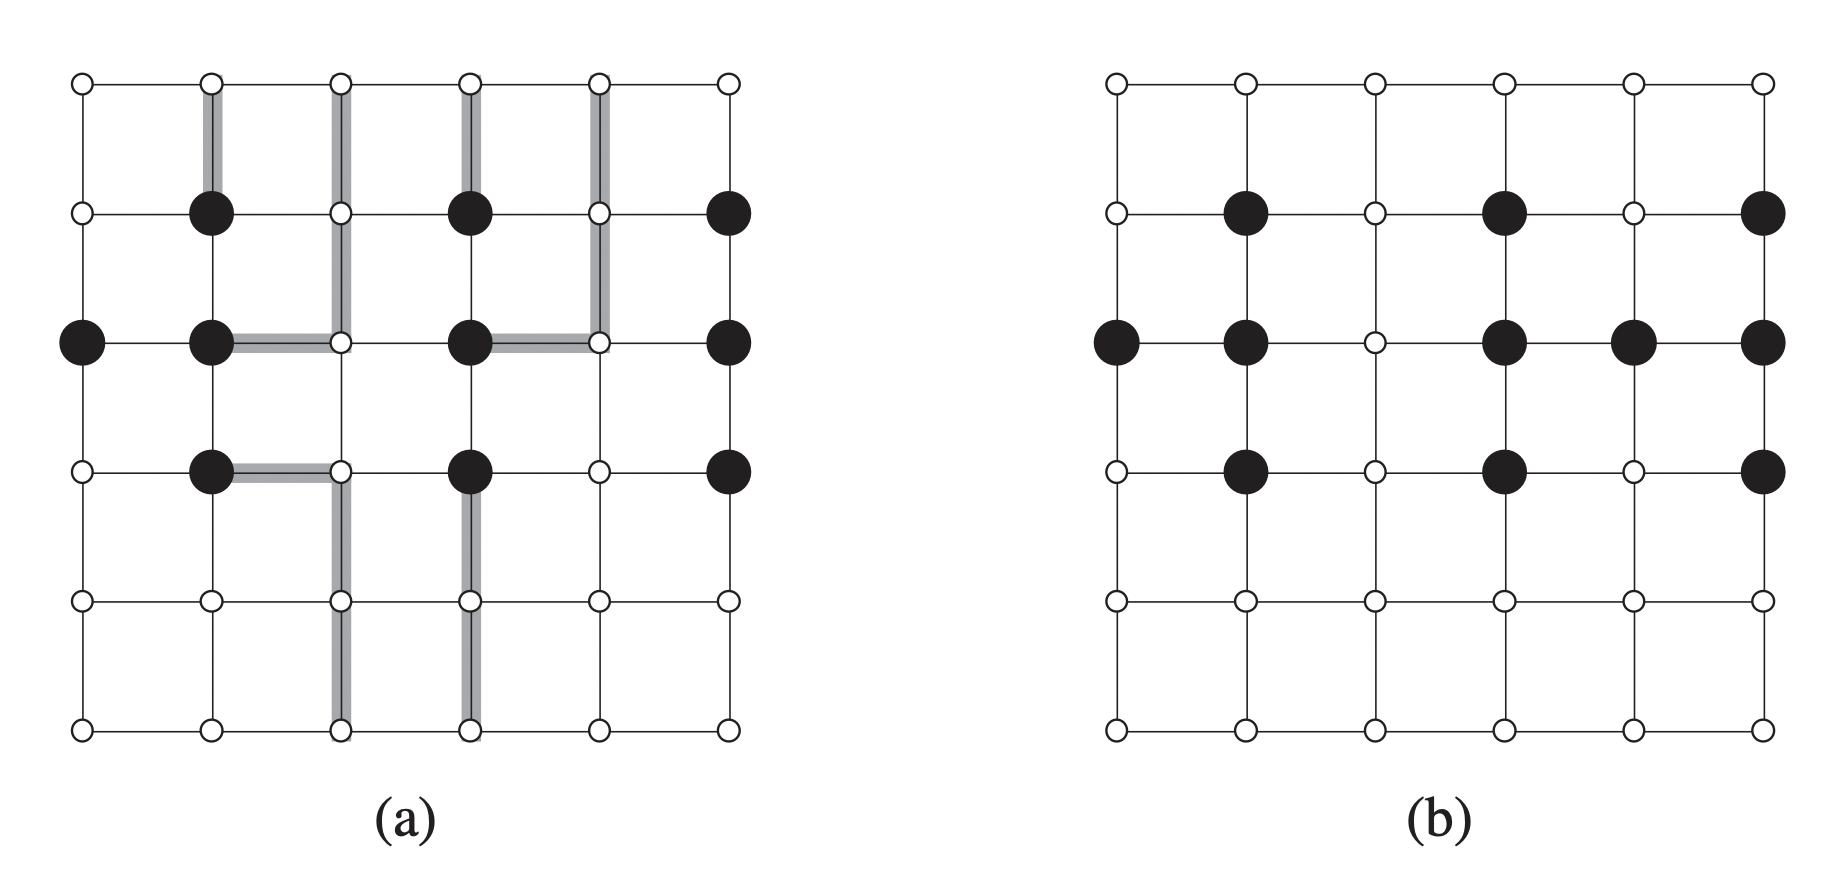
\includegraphics[width = 10cm]{img/1.png}
    \caption{Grids for the escape problem. Starting points are black, and other grid vertices are white. \textbf{(a)} A grid with an escape, shown by shaded paths. \textbf{(b)} A grid with no escape.}
    \label{fig:1}
\end{figure}
\begin{enumerate}[\textbf{\textit{\alph*.}}]
    \item Consider a flow network in which vertices, as well as edges, have capacities. That is, the total positive flow entering any given vertex is subject to a capacity constraint. Show that determining the maximum flow in a network with edge and vertex capacities can be reduced to an ordinary maximum-flow problem on a flow network of comparable size.
    \item Describe an efficient algorithm to solve the escape problem, and analyze its running time.
\end{enumerate}

\end{document}
